% Settings  (fold)
% State of The Art

\documentclass{llncs}

\usepackage[utf8]{inputenc}

%Separar os parágrafos
\parskip 2mm

\usepackage{acronym} %Acronimos
\usepackage{fnbreak} %Verifica se ha notas de rodape separadas
\usepackage{multirow} %Colunas grandes em tabelas
\usepackage{pdflscape} %Paginas em modo paisagem
\usepackage{paralist} %Inline lists
\usepackage{graphicx} %Imagens
\usepackage{comment}
\usepackage{color}
\usepackage{array}	% Tables
\usepackage{wrapfig}
\usepackage{bbding} % checkmarks and other symbols
\usepackage{hyperref}
\hypersetup{
	pdftex,%
    colorlinks,%
    citecolor=black,%
    filecolor=black,%
    linkcolor=black,%
    urlcolor=black,%
	bookmarks=true
}
\usepackage{bookmark}
\usepackage{subfigure}
\usepackage{subfigmat}


\newenvironment{myitemize}{
	\begin{itemize}
	  \setlength{\itemsep}{1pt}
	  \setlength{\parskip}{0pt}
	  \setlength{\parsep}{0pt}}{
	\end{itemize}
}

%\input{../commands.tex} %Inclui os comandos definidos no ficheiro
                        %externo

%Comando para inserir keywords no template da springer
%\newcommand{\keywords}[1]{\par\addvspace\baselineskip
%\noindent\keywordname\enspace\ignorespaces#1}
\renewcommand{\rmdefault}{phv}
\renewcommand{\sfdefault}{phv}

% (end)

\begin{document}
\pagenumbering{arabic}
\pagestyle{plain}


% ------ Nomes das propriedades ------ %
\newcommand{\alog}{Action Logging}

% ----- Acronimos --------%
\acrodef{UI}[UI]{user interface}
%\acronym{UI}{user interface}
\acrodef{SOM}[SOM]{self organizing map}
\acrodef{CBIR}[CBIR]{content based image retrieval}
\acrodef{MP}[MP]{megapixel}
\acrodef{FEP}[FEP]{Feature Extraction Plugin}

\acrodef{UX}[UX]{user experience}
\acrodef{WPF}[WPF]{Windows Presentation Foundation}
\acrodef{EXIF}[EXIF]{Exchangeable image file format}
\acrodef{HDR}[HDR]{High Dynamic Range}
\acrodef{SUS}[SUS]{System Usability Scale}


\newcommand{\todo}[1]{\textcolor{red}{TODO: #1}}
\newcommand{\red}[1]{\textcolor{red}{#1}}
\newcommand{\super}[1]{\ensuremath{^{\textrm{#1}}}}
\newcommand{\side}[1]{\marginpar{\textcolor{red}{#1}}}
\newcommand{\cm}{\Checkmark}
\newcommand{\fig}[1]{fig. \ref{fig:#1}}
\newcommand{\Fig}[1]{Fig. \ref{fig:#1}}
\newcommand{\hide}[1]{}


% \newcommand{\todoo[1]{\marginpar{\bf{\textcolor{red}{$\Rightarrow$ TODO:\\}}\scriptsize{#1}}}}


\title{Eagle Eye}
\subtitle{Visualizing large photo collections}

\author{Carlos Eduardo H. J. Fonseca}
\institute{
Universidade Técnica de Lisboa\\
Instituto Superior Técnico\\
Av. Rovisco Pais\\
Portugal\\
\email{carlosefonseca@ist.utl.pt}\\
2010
}

\maketitle

\begin{abstract}
	Digital photography has been a part of people's lives for the past decade, growing on hard drives, but image visualization has not been evolving enough to accompany this growth. Most people keep photos on folders or use software that can't display a large number of photos at the same time, not providing a good overview of their collection.

	This work grew from the features of other works of alternative image visualizations and tries to bring a better way for regular people to explore their photo libraries and learn more about them.

	This work provides an extensible backend system intended for image and metadata processing, gathering information about the user's photos, currently colors, faces, dates, paths and keywords, but, since it's extensible, could be used for much more.

	We also created a visualization application to use the processed data and provide it to the users, in an interface that is clean and simple. It starts by displaying all the added images on the screen, at the same time, in a grid, grouped by dates. From here, the user can zoom in and out and change the display to organize the images by colors, faces or paths, and can filter using a mix of any data gathered by the backend . This way, users can view and explore their libraries in a different way from what they have been doing.
	
\end{abstract}

%\keywords{organisational Engineering, organisation Redesign, Action Capture}


\chapter{Introduction} % 5/6 pages
\label{chapter:introduction}


\section{Prologue} % (fold)
\label{sec:prologue}

Since the advent of digital photography, people have been storing their photographs on folders on their computers instead of photo albums on the self. One could say computers can help people view, explore and find more photos in a shorter period of time, they certainly have the power for that but, in fact, they really don't do anything else then make the user look for the photo album (probably a folder or an ``album'' on some applications) and then flick through its pages (scrolling) until the photos that he was looking for appear.

This is true for the most common photo management software, like Google's Picasa\footnote{\url{http://picasa.google.com}}, Apple's iPhoto\footnote{\url{http://www.apple.com/iphoto}} or Aperture \footnote{\url{http://www.apple.com/aperture}} or Adobe's Lightroom \footnote{\url{http://www.adobe.com/lightroom}}. Although they bring some management improvements with them, the analogy above still applies. They all provide a way to select albums or folders and scroll through contents. They allow searching through some metadata and have lots of buttons and options for their editing capabilities.

We want to provide the user a totally different way to interact with his photos by focusing only on them. We want to provide the user a birds-eye view of his photos by showing everything and allowing him to drill down and view any image he wants at a larger size. Eagle Eye is not meant to be an editing platform but a better visualization tool.

With this work we will show that \red{this is a good alternative way to look at the users photo collection and that the user can learn more things from it}.


% section prologue (end)


\section{Context} % (fold)
\label{sec:context}


Present concepts...?
% section context (end)


\section{Motivation} % (fold)
\label{sec:motivation}

Alguns casos de uso

\chapter{Related Work}
\label{chapter:related-work}

% Should be around 20 pages

Interactive image visualization techniques have been explored for some time now, many of them related to image organization or retrieval in large collections. There have been some interesting ideas across the board and we will now take a look at some of them.


\section{Related work}

\subsection{Visual guided navigation for image retrieval} % (fold)
\label{sub:Qiu}

Qiu et al. \cite{Qiu:2007p1207} explore the requirements of a system intended for visualizing large photo collections. They identify as the two most important requirements, the first being an easy to use \ac{UI}, that gives clean information to the user and helps to create a mental image of the whole collection helping him to navigate on the collection. The second requirement is responsiveness because while image processing can be an heavy task, the user needs to be able to interact with the interface and he won't use the application if it's slow. 

\begin{figure}[ht]
	\centering
		\includegraphics[width=0.6\columnwidth]{imgs-RelatedWork/Qiu-2007p1207.png}
	\caption{The chromacy diagram is split in parts and each image belongs to one of this parts. The diagram is part of the \ac{UI} and  when navigating through the diagram, only the images related to that part are shown.}
	\label{fig:qiu1}
\end{figure}

The system shows all the photos arranged by color, just as many others like it. The difference is the process in use. Instead of calculating distance vectors based on the histogram of each image, this approach classifies each image with a simple description, like a mean of its colors, and arranges them by that value, on a color map (\fig{qiu1}). The process is much faster but is also more error prone, specially on photos without a clear main color.

Their tests show they achieved good responsiveness and better results than using a file explorer.

% section Qiu (end)

\subsection{Does organization by similarity assist image browsing?} % (fold)
\label{sub:Rodden}
\begin{figure}[ht]
	\centering
		\includegraphics[width=\textwidth]{imgs-RelatedWork/Rodden1}
	\caption{Three arrangements of 100 images of Kenya, based on visual similarity. On the left is the arrangement with overlap, in the middle a 12x12 grid (which removes the overlap while preserving some of the structure), and on the right a 10x10 grid (which maximises the thumbnail size).}
	\label{fig:Rodden1}
\end{figure}

The aim of this work by Rodden and Sinclar \cite{Rodden:2001p731} was to evaluate how photo organization by similarity (\fig{Rodden1}) could benefit a user looking for images. Some users tested an application that could show the same images both in a random and in an organized by similarity way. This organization by similarity was based on a rough description of the images but it could be other descriptors.

The results differ if the user knows what he's looking for or not. In case he does, being able to filter only the relevant images makes it quick to find the ones that matter. This obviously depends on the quality of the labeling. Users reported that sometimes the similar images appear to merge.

In case the user doesn't know what he's looking for, the random approach might be helpful because the strong images usually contrast to their neighbors and thus appear to stand out.

For some people, having access to different arrangements of the same set of images is useful, although the source of the individual differences still needs to be determined.

% section Rodden (end)


\subsection{Browsing large collections of images through unconventional visualization techniques} % (fold)
\label{sub:Porta}

\begin{figure}[!htb]
  \begin{subfigmatrix}{2}
    \subfigure[Spot display]{\includegraphics[width=0.49\linewidth]{imgs-RelatedWork/Porta-spot}\label{fig:porta-spot}}
    \subfigure[Shot display]{\includegraphics[width=0.49\linewidth]{imgs-RelatedWork/Porta-shot}\label{fig:porta-shot}}
  \end{subfigmatrix}
  \caption{The two better visualizations from Porta's work.}
  \label{fig:porta}
\end{figure}


Porta \cite{Porta:2006p416} describes a few visualization methods for large collections of images and tests them with users. The purpose it to find ways or metaphors that provide a good visualization experience in terms of time spent and quality of the visualization.

Some of the various techniques were the simple image grid view, a grid view with variable and independent height and width (EIB), a view that animates images like they were shot from a distance and get closer to the user called Shot (\fig{porta-shot}), a view where images quickly appear on random positions on screen named Spot (\fig{porta-spot}), and some other less commons like one that simulates an cylinder created with images (Cylinder), and others less relevant (Rotor, Tornado and Tornado of Planes).

The testing was based on the efficiency of users searching for specific images on a collection of a thousand photos. The Spot view was the best, followed the Shot, Cylinder finally the common grid view. The other views got scores near or below the grid view.

% section Porta (end)

\subsection{A comparison of static and moving presentation modes for image collections} % (fold)
\label{sub:Cooper}

This paper by Cooper et al. \cite{Cooper:2006p543} is not about large libraries but about what kind of interfaces for image showing has greater success of user recognition and preference (\fig{Cooper1}).

With the help of eye-tracking techniques and user preference, the authors determined that static images are better than moving ones because makes them easier to recognize and avoid some user confusion.

\begin{figure}[ht]
	\centering
		\includegraphics[width=\textwidth]{imgs-RelatedWork/Cooper1}
	\caption{The six rapid serial visual presentation modes used in the experiments}
	\label{fig:Cooper1}
\end{figure}
% section cooper (end)

\subsection{Organizing and browsing photos using different feature vectors and their evaluations} % (fold)
\label{sub:Strong}

Although it doesn't mention why, Strong \cite{Strong:2009p413} focuses on the better experience provided by color organization of a large image collection (\fig{Strong1}).

A \ac{SOM} is used to display the images on the screen featuring zooming, panning and sorting capabilities. The work is then based around the various methods used to determine the images' similarity.

Simpler methods are based on color histograms, which aren't affected by rotations or scales but, by not having spacial information on colors, allows very different images be closer together.

Other methods rely on gradients which contain spatial information and, therefore, are sensitive to image contents but not color.
In general, the best methods were found to be the hybrid ones, where both color histograms and gradients are used to classify the images.
No user testing is made in this project, neither is the speed of image categorization referred about the methods used.

\begin{figure}[ht]
	\centering
		\includegraphics[scale=1]{imgs-RelatedWork/Strong1}
	\caption{The result obtained for organizing 2200+ photos using color autocorrelogram feature vector, using \cite{Strong:2009p413}}
	\label{fig:Strong1}
\end{figure}

% section strong (end)

\newpage
\subsection{An evaluation of color-spatial retrieval techniques for large image databases} % (fold)
\label{sub:Tan}
% não tem imagens

Tan et al. \cite{Tan:2001p850} present an evaluation of three color-spatial image retrieval techniques.

The signature-based technique creates a signature for each image, based on the most frequent colors, according to a threshold, of each subdivision, or bin, of that image. The comparison between images is made by comparing the main colors present on each bin. It is possible to assign more weight to specific bins according to the user's interest.

The partition-based approach is also based on bins, each having it's own color histogram. The similarity between images is given by the distance of the histograms of the corresponding bins.

The cluster-based method bases on the fact that humans focus on large patches (clusters) of the same color and, therefore, two images will appear similar if both have similar colored clusters on at roughly the same location. This method extracts the larger clusters and their color from each image. The similarity is calculated by the amount of overlap between clusters.

This techniques were tested with a collection of 12,000 images and, besides the color information, the brightness was also analyzed for increased performance. The authors conclude the signature method was generally better on both effectiveness and efficiency.

% section tan (end)

\subsection{Automatic organization for digital photographs with geographic coordinates} % (fold)
\label{sub:Naaman}

In this paper, by Naaman et al. \cite{Naaman:2004p1802}, is described a system that organizes digital photographs accordingly to location and date embedded on the metadata.

The objective was trying to mimmic the the way people think about their collections. Photos are usually bursts separated by some time. Based on this and on the different places, events can be created to agglomerate photos from the same bursts. Location naming is done by calculating the most relevant places, like parks or cities, and then mixing the more precise locations with the more important neighbor cities to create a relevant and identifiable name. This was specially important since this work didn't involve showing any maps but only the location names and events.

The authors showed good results and, nowadays, some common applications use similar features although including maps.
% section naaman (end)

\subsection{Similarity pyramids for browsing and organization of large image databases} % (fold)
\label{sub:Chen}

Chen et al. \cite{Chen:1998p2344} present a method for designing a hierarchical browsing environment called a similarity pyramid. The similarity pyramid groups similar images together while allowing users to view the database at varying levels of resolution. Each level is organized such that similar images are in close proximity on a two-dimensional grid (\fig{Chen1}). Images are first organized into a binary tree through agglomerative clustering based on color, edge and texture similarities. The binary tree is transformed into a quadtree, a tree in which each node has four children instead of only two.

\begin{figure}[ht]
	\centering
		\includegraphics[scale=0.8]{imgs-RelatedWork/Chen-1998p2344.png}
	\caption{Images organized with \cite{Chen:1998p2344}. Images with similar color and texture are spatially adjacent.}
	\label{fig:Chen1}
\end{figure}

The similarity pyramid is best constructed using agglomerative (bottom-up) clustering methods, and a fast-sparse clustering method is presented which dramatically reduces both memory and computation over conventional methods. This method is based on the flexible agglomerative clustering algorithm, but using only a sparse proximity matrix and exploiting the author's approximate branch and bound search algorithm.

The authors found that the method for mapping the clustering to a pyramid can make a substantial difference in the quality of organization. Finally, a dispersion metric for objectively measuring pyramid organization was proposed, and found that it correlated well with the author's subjective evaluations of pyramid organization.

% section Chen (end)


\subsection{NN\super{k} networks for content-based image retrieval} % (fold)
\label{sub:Heesch}

Heesch \cite{Heesch:2004p2675} describes a different interaction technique for content based search in large image collections. Each image is a vertex in a graph and arcs are established between images if there exists at least one combination of features for which one image is retrieved as the nearest neighbor of the other. Each arc is weighted by the proportion of feature combinations for which the nearest neighbor relationship holds. By integrating the retrieval results over several feature combinations, the resulting network helps expose the semantic richness of images.

The interface reflects the vertexes and respective arcs, allowing to browse between the related images (\fig{heesch1}) in the network.

\begin{figure}[ht]
	\centering
		\includegraphics[scale=1]{imgs-RelatedWork/Heesch-2004p2675}
	\caption{Local network around the chosen butterfly image depicted in the middle.}
	\label{fig:heesch1}
\end{figure}

Seven low-level features are used for the classification of the images. HSV Global color Histograms maps the images by color, saturation and brightness; color Structure Descriptor maps the distribution of colors by dividing each image in 64 windows, the color space in 184 bins and associating color bins with image windows; Thumbnail feature compares identical images by saving the grey value of each pixel from a scaled down version of the image; Convolution filters discovers very selective features by reapplying 25 filters three times; Variance feature calculates standard deviations within a sliding window; Uniformity Feature is another statistical feature, calculating the grey level of an image split in 64 parts; Bag of words is the last feature and weights words associated to each image.

Tests showed great results using a mix of search, relevance feedback and browsing, and even only browsing was considerably better than other, more restrictive, approaches.

The technique helps avoid the problem of image polysemy by showing all gathered meanings of the images to the user.
The feature network is pre-computed, allowing for quick realtime browsing. The authors claim it took 50 hours to process 32000 images but made no reference to the possibility adding images to the collection, after the computation.

% section heesch:2004p2675 (end)

\subsection{Phorigami: A Photo browser based on meta-categorization and origami visualization} % (fold)
\label{sub:Hsu}

Hsu et al. \cite{Hsu:2009p2696} try to ease the browsing problem by analyzing the collections and identifying groups of related pictures. Each type of group is visualized in a specific way, inspired by the Origami art.

Groups of similar or related photos were manually classified based on camera movement and subject movement, creating different types of groups static view where both camera and subject are fixed and is presented as a panorama; multi-view where the subject is fixed but the camera is moving and is shown as a presentation; if the subject is moving, the photos are categorized as motion capture and can be shown as an animated photo (fixed camera) or a presentation (moving camera); finally group photos, where different groups of people are photographed, are shown as a folding presentation.

This covers various cases where the photographer takes a few similar photos of the same subject because it's either a panorama, various angles or just to be sure the photo was well captured. 

The interface implements the different presentation types as different metaphors, easy for the user to understand, like a folded paper on a wide panorama that can be expanded (\fig{hsu1}). Although some of them appear to be a little hard to distinguish in its compressed form, it shouldn't be difficult to make it clearer. Other possible problem is the use of different touch interactions for each presentation type that might confuse users on what gesture should they use.

\begin{figure}[ht]
	\centering
		\includegraphics[width=\textwidth]{imgs-RelatedWork/hsu.png}
	\caption{On the left, an example of an interaction on a group of photos that makes a panorama. On the right, a visualization on 537 photos with some groups.}
	\label{fig:hsu1}
\end{figure}


% section hsu:2009p2696 (end)

\subsection{A next generation browsing environment for large image repositories} % (fold)
\label{sub:Schaefer}

\begin{figure}[ht]
	\centering
		\includegraphics[scale=1]{imgs-RelatedWork/shaefer1.pdf}
	\caption{Hue sphere of a dataset}
	\label{fig:schaefer1}
\end{figure}

Schaefer \cite{Schaefer:2010p1871} tries to take similarity based organization of images from the 2D space to a 3D sphere, which allows interaction from the users. Rotating the sphere reveals images with different colors while tilting it reveals brighter or darker images.

Large image collections are handled through a hierarchical approach that brings up similar, previously hidden, images when zooming in on an area.

The description of the color is retrieved by calculating the image's median color for it's efficiency over other methods like histograms. This two features are directly mapped onto the sphere's coordinates and the entire structure is pre-calculated so browsing can be performed in real-time. Image overlapping is also avoided (\fig{schaefer1}).

The work was tested on a 4500 image collection with no evaluation as to its performance and a weak and subjective user testing.


% section schaefer:2010p1871 (end)

\subsection{Flexible access to photo libraries via time place, tags, and visual features} % (fold)
\label{sub:Girgensohn}
\begin{figure}[ht]
	\centering
		\includegraphics[width=\textwidth]{imgs-RelatedWork/Girgensohn1.pdf}
	\caption{Photos Grouped by Geographic Similarity and Filtered by Date and Place.}
	\label{fig:girgensohn}
\end{figure}

MediaGLOW by Girgensohn et al. \cite{Girgensohn:2010} is the application discussed in this paper. It's a \ac{CBIR} system with multiple ways to filter and sort the image collection.

The interface allows selecting a range of dates, places and tags at any time to filter the collection and the display will show the photos that match the filters, alongside indications of the existence of photos that match some of the filters. This display can then be arranged by four similarity criteria: temporal (by photo creation time), geographic (distances between places), tags (photos with similar tags are shown closer together) and visual (\fig{girgensohn}).

The time is selected using a timeline on the top of the screen while tags and places are shown on the right side sorted alphabetically, by frequency of, in case of places, as a tree. Multiple selections are allowed to show more photos.

The photo display is graph based, allowing for overlapped images. Various metaphors were developed to ease the navigation of the collection. Zooming is allowed and changes both thumbnail positions and size for better experience, allowing the photos to spread away from each other but also increasing the size so the user can have a better look at them. The authors think that bigger thumbnails and a correct grouping of related photos is more important than spreading them to avoid the overlapping problem.

Color coding is used throughout the interface to help the user understand better what is being selected. For instance, on the timeline blue and grey are used to distinguish photos that match or not the selected location/tag. On the photo display, besides the photos that are actually shown are colored blocks: blue for photos that match location only, green for time only and grey for those that didn't match anything.

Detailed user testing was performed and the importance of the multiple ways to organize and search the collections was emphasized since many systems are designed to have a single form of access. Some users also pointed the importance of being able to have a non overlapping view of the photos for part of the task.

Each view was found to have different levels of usage, the geographic being the most used and temporal the least, since it's very similar to the timeline. Visual similarity was less used than expected, even on collections where it was relevant. 




\subsection{PhotoMesa: a zoomable image browser using quantum treemaps and bubblemaps}
\label{sub:PhotoMesa}

This work presents PhotoMesa by B. B. Bederson \cite{Bederson:2001:PZI:502348.502359}, an application that supports browsing sets of images in a zoomable environment. It also supports clustering by metadata, not requiring previous work from the user. Users can choose directories of images and they are all displayed in a space-filling manner \fig{photomesa}. Images are displayed in groups, from the directories they origin from and users can smoothly zoom in to a group and then to a single image. It generates multiple-resolution thumbnails for maintaing a good performance. Keyboard keys are also used to navigate the canvas. The groups display their name and have different background colors for a better distinction. It also supports drag and drop of images to other applications. Text search is possible as well as selecting a group on a list.

\begin{figure}[ht!]
	\centering
		\includegraphics[width=0.90\textwidth]{imgs-RelatedWork/PhotoMesa.pdf}
	\caption{PhotoMesa with over 500 images in 17 groups.}
	\label{fig:photomesa}
\end{figure}

PhotoMesa implements two algorithms for space filling, one is Quantum Treemaps by the author, a variation of the Ordered Treemap  that is aware of the constraints imposed by the use of images, like grid alignment and common size, and Bubble Maps which is designed to have the least wasted space possible.

This work brings very interesting ideas to the table but it has a somewhat limited reach, with only referring to ``over 500 images'' on the application and by only taking simple metadata, like the path and modification date of images.




% section girgensohn:2010 (end)

\section{Discussion} % (fold)
\label{sub:discussion}


Currently there are a lot of approaches to image organization and each has its own differences as demonstrated on Table \ref{tab:brows-meth}. Our survey went by multiple works and revealed various methods for extracting the features from each image, multiple visualization methods from grids to flying images.


\begin{table}[ht]
\caption{Different browsing methods}
 \begin{tabular}{| m{2.7cm} |>{\centering}m{2.3cm}|c|c|c|>{\centering}m{2.1cm}|>{\centering}m{2.3cm}|r|}
  \hline
\multirow{2}{*}{\textbf{Work}} & \multicolumn{4}{c|}{\textbf{Organization}} & \multirow{2}{*}{\textbf{Visualization}} & \multirow{2}{*}{\textbf{Focus}} & \multirow{2}{*}{\textbf{Size}} \\
\cline{2-5}
	& \textbf{features} & \textbf{date} & \textbf{gps} & \textbf{tags} & & & \\

\hline 1.	Qiu \cite{Qiu:2007p1207}	& simple color measures 			& --- & --- & --- & Grid 			   & Simplicity and Efficiency 			& 60,000	\\
\hline 2.	Rodden \cite{Rodden:2001p731}	& --- 								& --- & --- & \cm & Grid 			   & Similarity usefulness	 			& 	 100	\\
\hline 3.	Porta \cite{Porta:2006p416}	& --- 								& --- & --- & --- & Spot (and others)  & Unconventional visualizations		& 	 400	\\
\hline 4.	Cooper \cite{Cooper:2006p543}	& --- 								& --- & --- & --- & Static and animated& Usefulness of animations 			& 	 ---	\\
\hline 5.	Strong \cite{Strong:2009p413}	& color histograms and gradients 	& --- & --- & --- & \ac{SOM} 		   & Evaluation of different features	&  2,200 	\\
\hline 6.	Tan	\cite{Tan:2001p850}		& color histograms of subdivisions & --- & --- & --- & --- 			   & Evaluation of different features 	& 12,000 	\\
\hline 7.	Naaman	\cite{Naaman:2004p1802}	& --- 								& \cm & \cm & --- & --- 			   & Organization based on events 		& 	   N/A	\\
\hline 8.	Chen	\cite{Chen:1998p2344}	& colors, edges and textures 		& --- & --- & --- & --- 			   & Efficient fast-sparce clustering 	& 10,000 	\\
\hline 9.	Heesch	\cite{Heesch:2004p2675} & six different features 			& --- & --- & \cm & Radial 			   & Complex similarity network 		& 32,000 	\\
\hline 10.	Phorigami, Hsu	\cite{Hsu:2009p2696}	& --- 								& --- & --- & --- & Grid with groups   & Interaction on grupped photos 		&  1,333 	\\
\hline 11.	Schaefer \cite{Schaefer:2010p1871} & color histograms of subdivisions & --- & --- & --- & 3D Sphere		   & 3D mapping and interaction 		&  4,500 	\\
\hline 12.	MediaGLOW, Girgensohn \cite{Girgensohn:2010}	& --- 								& \cm & \cm & \cm & Overlapped graph   & Having the best way to find photos &    450	\\
\hline 13. PhotoMesa, Bederson \cite{Bederson:2001:PZI:502348.502359} & --- & \cm & --- & \cm & Q. Treemap / Bubblemap & Zoomable browser & 500	\\
\hline
 \end{tabular}
\label{tab:brows-meth}
\end{table}

One of the main problems is obtaining useful information from low level feature extraction of the image contents. Some try to get the most out of each image, with a variety of complex and time consuming procedures, e.g., a variety of methods based on color histograms \cite{Strong:2009p413,Tan:2001p850,Chen:1998p2344,Schaefer:2010p1871} or even more detailed ones with textures and convolution filters \cite{Heesch:2004p2675}. Others try to focus on avoiding the complex computations by only getting simple but somewhat useful information \cite{Qiu:2007p1207}. To contrast with these methods, Girgensohn's work \cite{Girgensohn:2010} has found that users prefer other ways to filter the collection, like tags, dates and locations. Low level features are still used but they have to be kept to understandable and useful options.

Date and location are simple similarity measures and can be used to group the collections by events and locations like Naaman did on this work \cite{Naaman:2004p1802}. Current mainstream software like Apple's iPhoto\footnote{http://www.apple.com/iphoto} or Google's Picasa\footnote{http://picasa.google.com} are already doing it in a semi-automatic way.

Textual metadata like tags and descriptions are also widely used both on our survey \cite{Rodden:2001p731,Girgensohn:2010,Heesch:2004p2675,Bederson:2001:PZI:502348.502359} and on all mainstream software. The problem with tags and descriptions is that people usually don't assign them to their photos but that's not a problem we're interested here.

The visualization is the field with most variations and experimentations, like Porta's work \cite{Porta:2006p416} where multiple options were tested but only a couple of the most simple were considered useful. The 3D Sphere \cite{Schaefer:2010p1871} is also visually interesting but doesn't provide a better interface to the collection since it's based on a grid view but hiding many images on the far side of the sphere. The Phorigami work \cite{Hsu:2009p2696} introduces some interesting metaphors for reducing the space occupied by some groups of photos, but some make the visualization harder and could, therefore, be improved.

Girgensohn and Bederson's works are among the most interesting and relevant to our vision. MediaGLOW's \cite{Girgensohn:2010} visualization approach allows images to be organized by various features and to be filtered down, displaying matched photos alongside placeholders for photos that are only match partially. The timeline on the top is also very useful. It has some problems like image overlap and capacity for showing large collections, but the ideas are still interesting. PhotoMesa \cite{Bederson:2001:PZI:502348.502359} has a visualization style close to what we want from our work but its reach is short, i.e., has a small set of features and dispositions, doesn't handle many images and the \ac{UI} seems a little cluttered with all the strong colors and borders.

The seemingly more useful exploration tools are the ones that handle less images, which seems like a contradiction. The more images a system can hold and efficiently display, the more useful it gets. We want to suppport, at least, a few thousand images.

% section discussion (end)
% chapter related-work (end)
\chapter{Solution Requirements} % (fold)
\label{chapter:solution_requirements}

Our survey was based on various types of previous work from the last ten years. Image browsers and technology have evolved a lot since then, but there still isn't a definitive way for a user to look at his larger photo collection and understand its content and evolution.



We have the vision of a system that displays a large set of user’s photos at the same time, in various arrangements, revealing patterns, differences and similarities between them.

We will now expose this vision by presenting the main goals we want to achieve with this thesis, as well as some of the guiding implementation requirements that we followed for a better end result.





\section{Main Goals} % (fold)
\label{reqs:main_goal}

The main goal of this thesis is to provide a different approach to the photo collection browsing methods. More specifically, the work should:


\subsubsection{Extract interesting information about the images}
We want to be able to organize and classify images. As we have seen on the Related Work, there are many ways to extract information from images, some simple, some complex. We have chosen a few that we think are the most relevant to the scope of our work. We will explain what we chose and why below, in section \ref{reqs:features}.


\subsubsection{Provide an interaction with the full set of images}
We want to enable the users to easily view and interact with the all the images at the same time, if they want to, instead of just limiting to a small window of images. Many of the Related Work did this and displayed all images at the same time \cite{Qiu:2007p1207,Chen:1998p2344,Girgensohn:2009:MOP:1502650.1502711,Bederson:2001:PZI:502348.502359}. Others only displayed a subset of images, but we think the users should have the power to create and view their own subsets from the full one.


\subsubsection{Efficiently display a large number of images in a single screen} % (fold)
This goal goes inline with the previous one: to be able to interact with a large set of images, we should be able to display them all, at the same time, using techniques to make better use of available screen space. We saw different ways to display images on the Related Work, some focused on displaying images efficiently \cite{Qiu:2007p1207,Rodden:2001p731,Naaman:2004p1802,Hsu:2009p2696,Bederson:2001:PZI:502348.502359}, others more focused on the relations between the images \cite{Girgensohn:2009:MOP:1502650.1502711,Heesch:2004p2675}. Hsu's work \cite{Hsu:2009p2696} is specially interesting for its idea of merging images that were related and we want to include this in our work, but with an automatic way of grouping and a clearer \ac{UI}.

\subsubsection{Allow the manipulation of the display}
We want the users to create different views that enable new perceptions of their collection, based on the extracted information. Many works allowed some sort of highlight \cite{Girgensohn:2009:MOP:1502650.1502711}, zoom \cite{Bederson:2001:PZI:502348.502359} or similarity filter \cite{Qiu:2007p1207,Heesch:2004p2675}. Some are more useful then others and we think we should apply them sensibly. Since we are going to display a large amount of images at a small size, there will be the need to increase the size of the images, therefore we require the ability to zoom in on images and to provide some filters for any available data, but also for custom user selections. It is also interesting to have some similarity filtering.
	
\vspace{\baselineskip}
	
With this capabilities, our work should be able to provide the user not only a better understanding of the collection, but also with an easy and interesting way to visually combine and view photographs.


%be able to handle thousands of images and display them all on the screen while maintaining responsiveness and giving useful information. The system's \ac{UI} should be clear and easy to use, allowing the user to navigate through the display of photos, through zooming and panning, and to reorganize the display the photos in a number of ways.

%The system should also gather as much information as it can from the photos, such as date and time, relevant colors, presence of people, type of photograph, user organization or location. While some of this information is already embedded in today's digital photographs as metadata, written by the digital camera when the photo was taken, others are usually not and need to be calculated or extracted. Faces and relevant color information are an example of that and the system must be prepared to extract this features from the image. The system must provide some capability for other feature extraction methods to be easily added in the future. All this information will then be used by the user to reorganize and filter the photos on display.


%§ We will now detail the work done, taking this requirements into account.

% subsection main_goal (end)









\section{Implementation Requirements} % (fold)
\label{reqs:Implementation_Requirements}

In addition to the referred main goals, we set ourselves some design goals, or requirements, for our implementation. With them, we want our work to get closer to a real application, that real users can use and have some flexibility for it to evolve with time.

Therefore, we set the following requirements:

\subsubsection{Ease of Use} % (fold)
\label{reqs:ease_of_use}

Ease of use is one of the most important characteristics of any piece of software and can shape how well it will sell. Much more attention has been given to the \ac{UX} in the last few years. Systems that are easier to use, get the job done faster, are more enjoyable to use and allow less experienced users to use them.

Since this is such an important characteristic, we aimed at providing a simple interaction from the beginning to the end, while also providing a powerful system, even though it could be even more refined in a few areas.

% subsubsection ease_of_use (end)



\subsubsection{Extensibility} % (fold)
\label{reqs:Extensibility}

The extensibility factor of a system is also important for the added value that can be obtained by quickly adding new features, either by the developers or by third parties. We made some parts of our work with this in mind, by allowing either external plugins or by generalization of code, allowing for future improvements with less trouble.

% subsubsection Extensibility (end)



\subsubsection{Performance} % (fold)
\label{reqs:Performance}

One of our main goals is to display a large set of images on the screen, but this brings problems since each image, in full-size, can take a good set of resources of the system. If we multiply this resources for a thousand images, we will not have a performent work.

Therefore, we set this requirement for having a performent work, that can be used with at least a few thousand images without taking down the system while using it.
% subsubsection Performance (end)




\subsubsection{Persistency}

Our system will spend sometime generating and gathering data for each of the available feature extractors, for each image. To avoid having to re-do work in case of a failure, addition of more images to the collection or stopping to resume later, the system must store the data after its generation. This should be accomplished using a system wide framework to provide easy storing of all the data. Since this work is intended to be an exploration of visualization concepts, so we will not support interoperability from our system to others by using MPEG-7 or other metadata descriptor standards, but instead use something that is simpler to implement.


% subsection design_goal (end)




\section{Features of Images and Photographs}
\label{reqs:features}

%extract interesting information about the images
As referred before, we want our system to extract interesting information about the images and we will now explain this in detail.


Unlike textual data, images are a type of data where is not trivial to extract information from, in a computational environment. It's easy for us, common people, to understand what certain picture is showing. We can easily distinguish if there are, for instance, animals, people, flowers or buildings, but it's hard for a computer to do the same, and it's even harder to understand if that certain photo of a building and a person was taken because of the building, the person or both.

There have been various developments in the feature extraction front \cite{Liu:2007p3740,Datta:2005p3749,Rui:1999p949} and is currently possible to perform various detections in images with various levels of satisfaction.

Some examples of working solutions for feature detection:

\subsubsection{Face recognition}
Detection of the presence of faces in the images, their position and relations between them as some other works refer \cite{Vasconcelos:2005in,Chen:2003p3699,Tamura:2002p859,Hsu:2002p3675}. Face recognition has been gaining public appreciation in the past few years since many photo applications and services have been including it. Our user survey reflects that people like this feature and request it (\ref{:suggestions_of_features}). The problem with face recognition is that it requires users to identify who are the persons on each photo which, generally, is a long and repetitive process. For concept, we will only detect the presence of faces and not spend time identifying them.

\subsubsection{Object recognition}
Identification objects in images. This is a useful extractor, but is requires a huge library of sample imagery for comparison \cite{Torralba:2008p527} and it's not feasible to adopt in our work.
	
	
\subsubsection{Identification of perceptive colors}
What are the main colors that users perceive in certain image \cite{Sural:2002bt,Tan:2001p850}. An image is composed of different colors or tones and people can identify images by their main colors and dispositions. There are simple ways, like calculating the mean color for an image, but that's not faithful. Detecting perceptive colors identifies the different colors of an image, providing more realistic data.

\subsubsection{Image sequences}
Identification of images of the same scene that were taken in sequence, for grouping purposes \cite{Cooper:2003p3679}. Images taken in sequence of the same subject should be gathered into a group of images, with the purpose of reducing the needed space to display them. This is important since almost half of the people we inquired on our survey claims to use techniques that capture a great number of photos sequentially (\ref{ssub:photos_in_close_sequence}). This can be either by looking at the capture date or by analyzing the visual similarities of sequential images.

\subsubsection{Image similarity}
Identification of similar images across the whole collection enabling a search of similar images from a selected one or just grouping similar images according to defined parameters. There are many ways of doing similarity, some simple, like measuring the average color of the image \cite{Strong:2009p413,Qiu:2007p1207,Schaefer:2010p1871}, some complex like measuring various color attributes, edges, textures, applying filters or using convulsion like Heesch \cite{Heesch:2004p2675} and Chen \cite{Chen:1998p2344} did. For our work, we will explore options for color similarity, paving the way for other more accurate methods.

\vspace{0.5\baselineskip}

We want to use some of this methods to automatically extract information from the contents of images but, since this work is mostly focused on photography, there is another way to obtain really useful information that is EXIF Metadata. None of the related works seemed to use it, although users are interested in them, as can be seen on our user survey (\ref{ssub:preferred_features}\hide{ and \ref{ssub:suggestions_of_features}}).

EXIF Metadata is a standard format for metadata included in digitally captured media, like photographs captured by digital cameras. This devices save a lot of information on the image file, like the date and time of the capture, camera settings, camera orientation, location data and even detected faces\footnote{the availability of some of this data requires capable camera hardware and software that are getting more common nowadays.}. An example of the metadata fields can be seen on Table \ref{tab:exif}. This is textual data and, therefore, much faster and easier to retrieve and analyze than the content based methods we discussed above, being a great addition to them.

Mixing all this different data, users should be able to interact, filter, sort and organize their collection in various ways, obtaining new and different perspectives of their images.

\begin{table}[h]
\vspace{\baselineskip}
\renewcommand{\arraystretch}{1.4}
\rowcolors{2}{light-gray}{white}
\centering
\vspace{0.2cm}
	\begin{tabular}{ll}
	\textbf{Field Name}			&	\textbf{Example Value}\\
	\hline
	Camera:				&	Canon PowerShot S5 IS\\
	Exposure:			&	0.017 sec (1/60)\\
	Aperture:			&	f/3.2\\
	Focal Length:		&	6 mm\\
	ISO Speed:			&	80\\
	Exposure Bias:		&	-2/3 EV\\
	Flash:				&	Off, Did not fire\\
	Software:			&	Adobe Photoshop Lightroom 3.4\\
	Max Aperture Value:	&	2.7\\
	Subject Distance:	&	0.3 m\\
	Metering Mode:		&	Multi-segment\\
	Sensing Method:		&	One-chip color area\\
	Custom Rendered:	&	Normal\\
	Exposure Mode:		&	Manual\\
	White Balance:		&	Auto\\
	Keywords:			&	``Beach", ``Sand", ``Castles"\\
	Date and Time:		&	2010:09:18 11:52:59\\
	Lens:				&	6.0-72.0 mm\\
	Approximated Focus Distance:	&	0.3\\
	Flash Mode:			&	Off\\
	Metadata Date:		&	2011:06:14 20:03:04+01:00\\
	GPS Latitude: 		&	38 deg 52' 47.67" N\\
	GPS Longitude: 		&	9 deg 9' 47.13" W\\
	GPS Altitude Ref: 	&	Above Sea Level\\
	GPS Altitude: 		&	214.9 m\\
	GPS Date Time:		&	2010:09:18 10:52:59\\
\end{tabular}
\caption{Example of some relevant EXIF fields imprinted by the camera and by the computer software used for post processing.}
\label{tab:exif}
\end{table}



% chapter solution_requirements (end)
\chapter{Eagle Eye}
\label{cha:eagle_eye}

% 30/40 pages

Eagle Eye is the product of this thesis and is our implementation of the requirements previously detailed. It is a visualization tool that enables the display and manipulation of a large image set at once. It is focused at the regular computer user that has a few thousand digital photographs stored on the computer. It allows navigation, through panning and zooming of the canvas where the image collection is disposed, sorting in different ways while also allowing filtering, either textual or visual.

In this chapter, we will go through how does Eagle Eye work, what are its components and how they interact.


\section{Overview}

Our requirements stated the need for features to be extracted from images, so we  started by creating a system to enable that. We then changed our focus to the visualization part of the work and redefined the general architecture of the work. The system is now composed of two main elements: the Backend, which is the system that extracts features from the images and prepares everything to be displayed; and the Visualization which performs the display from the images and their extracted features to the user.


This is the overview of the system that we will now detail in the following sections.




\hide{


\section{Design Decisions} % (fold)
\label{sub:design_decisions}

\subsubsection{DeepZoom} % (fold)
\label{ssub:deepzoom}

After analyzing some visualization technologies that allowed easy display and manipulation of images \todo{Insert a bunch of ``useless'' tech}, Microsoft’s Silverlight, with its DeepZoom technology, proved to be the best choice.

DeepZoom enables the use of multiple resolution images for efficient display at various zoom levels and, for instance, is used for the display of gigapixel photos \footnote{Gigapixel photo of San Francisco: \url{http://theeyegame.com/DZSL/TwinPeaks5DMk2}}, where the user can view the whole image or zoom in the small details, or for collections of photos where the user can zoom between a view of multiple images and the details of a single image\footnote{Hard Rock Memorabilia: \url{http://memorabilia.hardrock.com}}. So far, usages of DeepZoom have been restricted to promotion websites, art galleries and other closed usages.

\red{This should be about the multi-scale images and not about DeepZoom $\rightarrow$ }Our work aims at bringing this technology to the regular user, in a much simpler and dynamic way.

Although DeepZoom seemed a great technology, it relies on Silverlight, which by itself isn't as good as using a full-fledged desktop application framework like \ac{WPF} or other frameworks native to their platforms. This created some undesired limitations like the need to have two separated parts of the system, the visualization and the backend, and other smaller problems like limited access to the disk from the visualization part.

To create a DeepZoom application, some pre-processing is required before hand to create multiple versions of each image in various resolutions and also to create imagery of a global view of the collection, also in multiple resolutions. This enables DeepZoom to only load the appropriate set of images for a certain zoom state, keeping the bandwidth (if used on the Internet) and memory requirements to a manageable level. This required pre-processing is done once on the backend. The visualization then uses the generated data to display the collection, being, at this point, totally independent from the original image files belonging to the user.

\subsubsection{Separation of Frontend and Backend}

As we just said, there's a need for previous processing to occur

% subsubsection deepzoom (end)
% subsection design_decisions (end)

}


\section{Backend} % (fold)
\label{sub:backend}

The backend is one of the two parts that make Eagle Eye. Its purpose is to extract information from images and set everything up for the Visualization.

Currently it is a command line utility that allows the user to enter paths for folders containing image files. The system will then read those images, gather their metadata, process them with the existing plugins to extract visual features and, finally, generate and output the multi-scale imagery and the control metadata required by the visualization.

We will now detail its architecture, and implemented feature extractors.

\subsection{Architecture of the Backend}

The Backend comprises a library manager to hold the images, feature extractors to process those images and persistence to save all generated data.

Figure \ref{fig:arch} is a simple explanation of the components. The Eagle Eye part is the main application, containing the library and feature extractor managers. Both deal with files on the disk, JPEG image files and DLL extractor plugins, respectively. The user interacts with the core of Eagle Eye which currently provides a command line interface for its actions, like the image import and plugin execution. The import gathers the files and their metadata, to be later accessed by the plugins for processing. Plugins store the resulting data inside the library manager and can be accessed afterwards for outputting by a special plugin.

We will now go through this components in more detail. 

\begin{figure}[ht]
	\centering
		\includegraphics[scale=0.7]{Figures/Architecture_v2.pdf}
	\caption{Basic architecture of Eagle Eye's backend}
	\label{fig:arch}
\end{figure}


\subsubsection{Library Manager} % (fold)
\label{ssub:library_manager}

The system displays images and, therefore, it needs to know what to show. This is where the library manager comes in. It creates a database which indexes existing JPEG image files stored on the user's computer and makes this information available for other modules to use. It is designed to be used with digital photographs which contain the aforementioned EXIF metadata like time, date, camera information, or location. This information is gathered upon import and is available throughout the Backend.

We explored a few ways to develop the image import process and we rested at the fastest we found. The user refers a folder to be imported and we use a third-party program, ExifTool\footnote{ExifTool is a utility that allows easy read and write of file metadata. \url{http://www.sno.phy.queensu.ca/~phil/exiftool}}, to crawl through the user-specified folders while identifying all the JPEG images and returning their \ac{EXIF} metadata which is then stored by our system (\fig{arch:import}).

\begin{figure}[ht]
	\centering
		\includegraphics[scale=0.6]{Figures/import.pdf}
	\caption{Process in use by our system for importing a folder using ExifTool.}
	\label{fig:arch:import}
\end{figure}


Another option for importing metadata was to invoke ExifTool as part of a \ac{FEP}. Although that could fix a couple of problems with the current  implementation, it doesn’t make the metadata as ubiquitous as needed. Most \acp{FEP} rely on some \ac{EXIF} plugins to work correctly and the current implementation doesn’t easily allow inter-\ac{FEP} data-sharing.

% subsubsection library_manager (end)




\subsubsection{Feature Extraction} % (fold)
\label{ssub:FeatureExtraction}

To enable the Visualization to arrange the images on the screen in different ways, they need to be classified. Some information is easy to obtain and compare, like when the photograph was taken. Other information needs to be extracted, like the number of people in the photo or what are the most relevant colors in the image. \Fig{fe} is a short example of what feature extraction is all about.

\begin{figure}[ht]
	\centering
		\includegraphics[width=0.72\columnwidth]{Figures/fe.pdf}
	\caption{Example of information extracted from an image.}
	\label{fig:fe}
\end{figure}

We had a few ideas for extracting features from images and, to be possible to add more along the way, we developed a plugin system to ease the creation of other feature extractors in the future.

Each Feature Extraction Plugin is separated from the main system. They need to implement a \red{common interface} and are given the ability to access the image data from the library, and save the computed data back. They have freedom to access the image file or its \ac{EXIF} information. They should, in the end, store the processed data in a specified way so it gets exported to the visualization. Implemented plugins will be explained in section \ref{sub:plugins}.

% subsubsection Feature Extraction (end)




\subsubsection{Persistence} % (fold)
\label{ssub:Persistence}

Persistence of both library and plugin data are required so the system doesn't lose information that took time to generate. To ease the interaction with a database system, we created a database abstraction layer that hides the complexities of interacting with said system. It also allows us to change to another database system if we see the need for it. We chose Oracle's Berkeley DB\footnote{Berkeley DB is a high-performace, embeddable, key-value, file-based database available at \url{http://www.oracle.com/technetwork/database/berkeleydb}} for its speed in retrieving data.

With this layer we can hide some optimization complexities like lazy-saving and lazy-loading. We use lazy-saving to save data to disk by chunks instead of doing it on each small update, speeding up the update process. Lazy-loading is not yet implemented, but it is essential with libraries with tens of thousands of images, where keeping a complete library in memory is not feasible.

% subsubsection database_abstraction_layer (end)

%subsection arch backend (end)












\subsection{Feature Extraction Plugins} % (fold)
\label{sub:plugins}

Back in the Solution Requirements chapter (\ref{reqs:features}), we detailed some possible features that were interesting to be used in this work. In this section we will detail what extractors have been implemented.

Currently, we have four feature extraction plugins:
\begin{myitemize}
	\item Selection of useful image metadata
	\item Detection of image’s main color
	\item Face detection
	\item Generation of multi-scale imagery
\end{myitemize}

We now proceed to the explanation of each one of this plugins. 

\subsubsection{Selection of useful image metadata}

This plugin acts as a filter for all the available \ac{EXIF} tags. It picks the most relevant ones, codes them in a pre-defined way and appends them to the rest of the information to be exported for the visualization.

Information when the photo was captured, what device was used, the path where it resides or information about the location where the photo was taken are a good examples of the most commonly relevant tags, as can be seen on the user survey (\ref{ssub:preferred_features}). In the future, this set of extracted tags could be optionally set by the user.


\subsubsection{Detection of image’s main color}

\begin{wrapfigure}{r}{0.3\textwidth}
	\vspace{-20pt}
	\begin{center}
		\includegraphics[width=0.29\textwidth]{Figures/parrot}
	\end{center}
	\vspace{-20pt}
	\caption{A colorful photo.}
	\vspace{-5pt}
	\label{fig:parrot}
\end{wrapfigure}

Sometimes people don’t recall where or when a photo was taken, or where is it, but they vaguely remember that the photo had some dominant colors, like the red of a parrot in a green background (\fig{parrot}). This kind of information can be helpful when searching for a photo in a collection.

Color extraction from images has been a long standing problem \cite{Wan:2011bg,Strong:2009p413,Gabbouj:2009en,Girgensohn:2009:MOP:1502650.1502711,Zaheer:2010p3735,Datta:2008p1604,Chang:2007bt}. We wanted to extract the most perceptible colors from images so, in the parrot example (\fig{parrot}), the system should associate the image with the colors red, green, white and black and avoid colors that have little relevance, like the small blue of  the feathers and also ignore small tonal variances in the reds and greens.

For that we explored two methods that reduce the number of colors in an image to the most essential ones, the first being an \textbf{adaptive method}, selecting a few averaged colors from the image and the second using a \textbf{predefined color palette} as reference to select the colors.

A common JPEG photo can contain 16.8 million different colors. Our adaptive method reduces the possible colors to less than ten\footnote{We tried with multiple options from one color to ten colors and the results vary from image to image. We think eight is a good value, keeping a nice set of colors on colorful images.}. The obtained colors are chosen by averaging the colors in the image, so if there's a lot of blue tones, a single, averaged blue will be replacing those tones (see the middle image of \fig{sky}). In areas that have little tonal variation of the color, the resulting color will be very similar to the original (like in the right image of \fig{sky}). But sometimes this method fails to save important colors when they occupy a relatively small area of the image or if the image doesn't have a strong contrasts (shown by the left image in \fig{sky}).

\begin{figure}[ht]
	\centering
		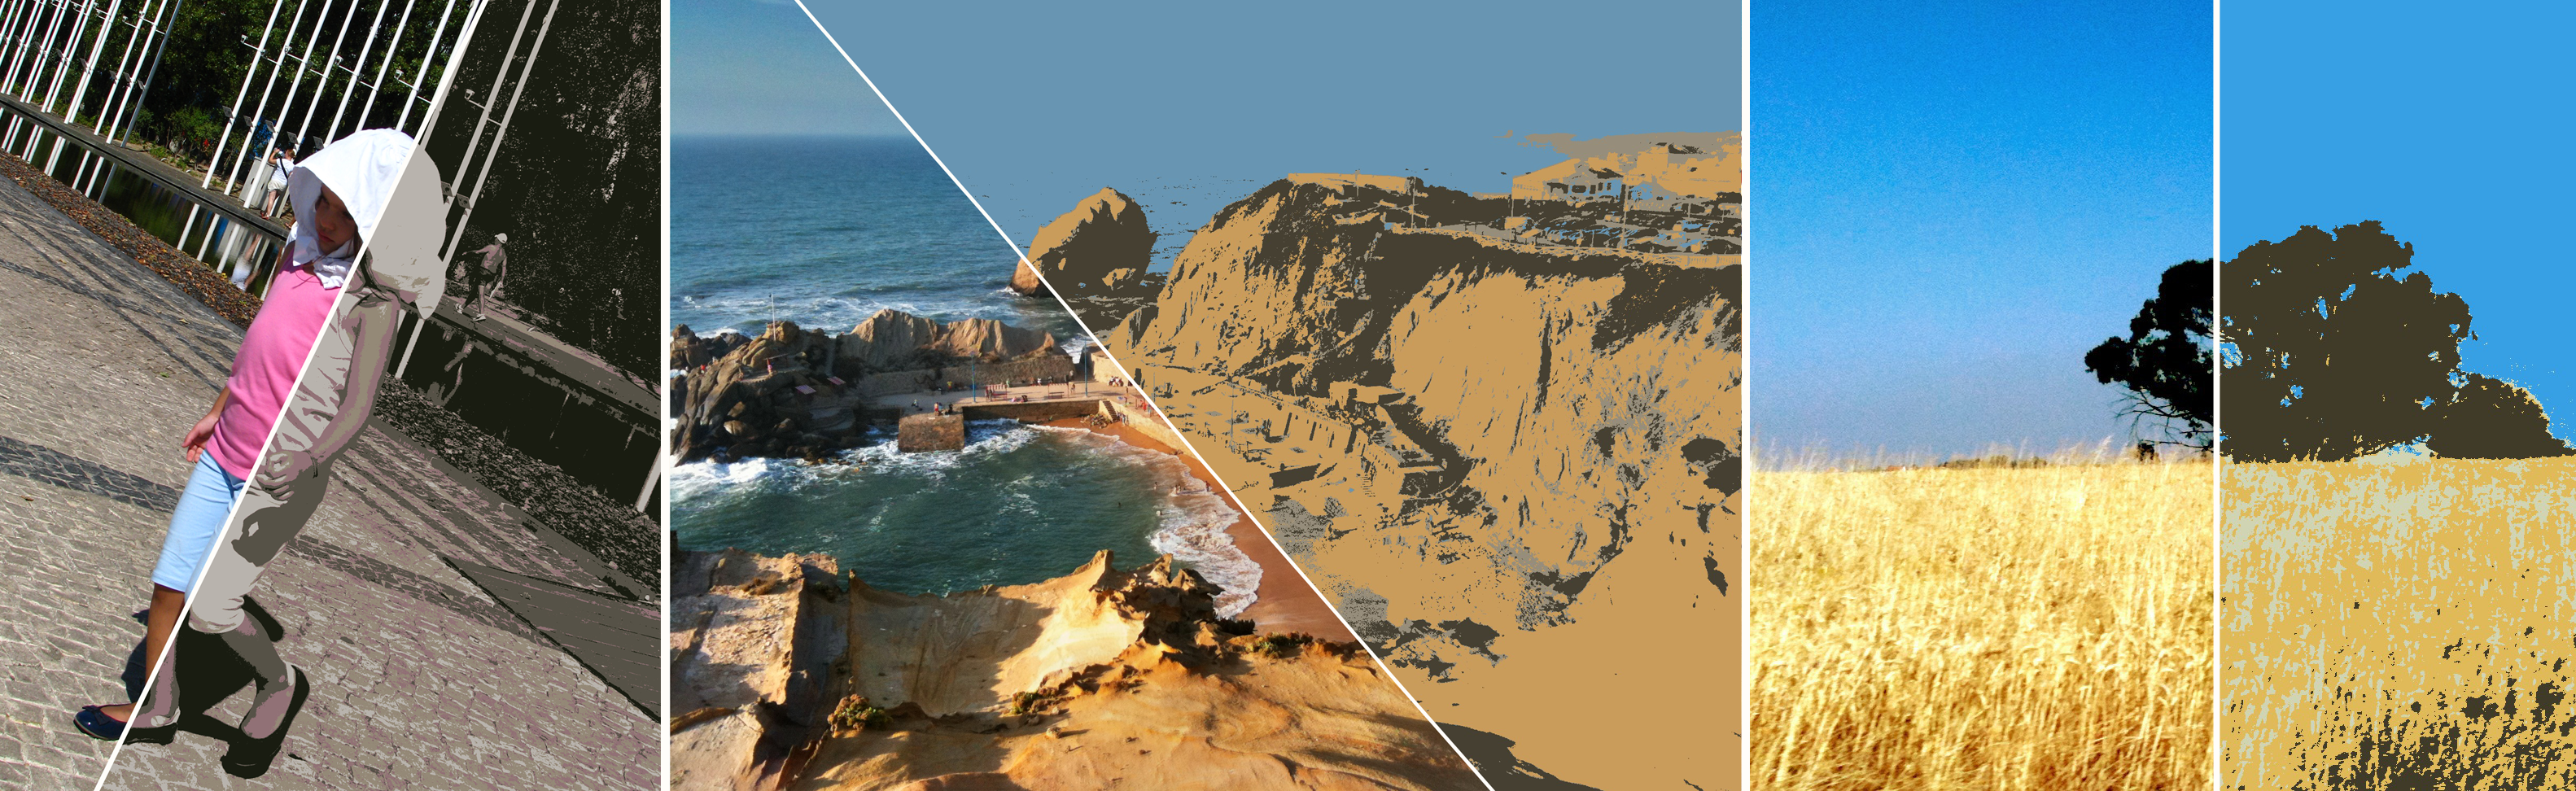
\includegraphics[width=\columnwidth]{Figures/colorreduction.png}
	\caption[Comparison of full color and reduced color images.]{Three images where the left half is the original version and the right half is a version with very limited number of colors provided by the adaptive method.}
	\label{fig:sky}
\end{figure}




The second method uses a predefined color palette (\fig{colors}) which is an adapted mix between the eleven most recognizable colors (red, yellow, green, blue, purple, brown, orange, pink, black, white and grey)\footnote{Qiu \cite{Qiu:2007p1207} explains these are the most universal recognizable colors in any language.} and the 21 ColorAdd colors\footnote{ColorAdd is a 21 color catalog with symbols for each color designed specifically for color blind people. We used the colors as a reference, specially the light and dark variations.}. This mix has a great range of colors and each one can be easily named with recognizable words\footnote{We want to avoid names like ``Amaranth'' or ``Munsell'' that most people don't know about. A large list of this names can be found on \url{http://en.wikipedia.org/wiki/List_of_colors}.} which then could be assigned to the images. The images processed with this method get their colors changed to the most similar ones present in our palette. This assures that colors in a relatively small area or images with low contrast still get the deserved attention (\fig{pinkP}), unlike the adaptive method (\fig{pinkA}). This method doesn't reproduce the colors so well as the adaptive but, since we want to obtain generic colors, this one is more reliable.


\begin{figure}[!ht]
	\centering
		\includegraphics[width=\columnwidth, height=45pt]{Figures/colours.pdf}
	\caption{Color palette in use for restricting the possible colors in an image.}
	\label{fig:colors}
\end{figure}


\begin{figure}[!htb]
  \begin{subfigmatrix}{3}
    \subfigure[Original image] {\includegraphics[width=0.328\linewidth]{Figures/pink1.png}\label{fig:pinkO}}
    \subfigure[Adaptive method]{\includegraphics[width=0.328\linewidth]{Figures/pink2.png}\label{fig:pinkA}}
    \subfigure[Mapping method] {\includegraphics[width=0.328\linewidth]{Figures/pink3.png}\label{fig:pinkP}}
  \end{subfigmatrix}
  \caption[Comparison between the original image, the adaptive color reduction method and the color mapping method.]{Comparison between the original image, the adaptive color reduction method failing to keep the pink and the blue colors and the color mapping method.}
  \label{fig:pink}
\end{figure}


This was the research we made to extract perceptible colors from images. We generated the above demonstration images using ImageMagick\footnote{ImageMagick is a software suite to create, edit, compose, or convert bitmap images. \url{http://www.imagemagick.org}} and its ``colors'' feature for the adaptive method and the ``remap'' for the palette method. Unfortunately, time was not on our side and we had to move to a simpler system. 

The current color extractor plugin does a simpler job of calculating the median color of the image and use the hue to index images.

We took some ideas from the work of Qiu et al\cite{Qiu:2007p1207} of exploring a method of image indexing that is fast and simple. On this work, images are sorted into ``bins'' according the their average color. This bins are divisions of color planes, indexed using binary trees allowing for very fast searches.

We used the open source library AForge.Imaging\footnote{AForge is a framework designed for developers and researchers in the fields of Computer Vision and Artificial Intelligence \url{http://www.aforgenet.com/framework/}} to obtain histograms for the images and compute their average color in RGB\footnote{Color model composed by red, green and blue \url{http://en.wikipedia.org/wiki/RGB}} and HSL\footnote{Color model composed of hue, saturation and luminance \url{http://en.wikipedia.org/wiki/HSL_and_HSV}} values. Both those values are then stored on the plugin-extracted data for each image. The images will be distributed into bins on the Visualization. We could assign bins at this point but, by not doing so, we are giving freedom to the users to change the number of bins used for display. We will discuss this on the Visualization sections ahead.


Although we didn't implement this plugin the way we desired, it demonstrates that color extraction is feasible and, with more time, a better method that does more than just averaging the colors, including detecting the most relevant ones, could be implemented.



\subsubsection{Face Detection} % (fold)
\label{ssub:face_detection}

The face detection plugin is based on the open-source OpenCV library\footnote{OpenCV (Open Source Computer Vision) is a library of programming functions for real time computer vision. Available at \url{http://opencv.willowgarage.com}} which processes every image file and detects existing faces (\fig{faces1}).
 
\begin{figure}[ht]
	\centering
		\includegraphics[width=\columnwidth]{Figures/faces1.jpg}
	\caption{Example of the OpenCV library detecting faces on a common photo.}
	\label{fig:faces1}
\end{figure}

No face recognition software is perfect. Usually if the software can detect every face, it will probably detect some other things in images that aren't faces (false positives). If it’s successful in only detecting faces, it will probably miss some other faces that aren't ideally positioned (false negatives). OpenCV is included in the latter, only detecting faces, but also missing some that are tilted (like in \fig{faces1}) or turned on the side.


This process is quite computationally expensive and therefore we resize all the images down to a more acceptable size, making the process more than five times faster.

We tested 29 images, from six different cameras, ranging from one to ten megapixels, and containing up to thirteen faces. The test consisted in running face detection on each image, in its original size and in various resolutions from 2000 to 200 pixels on its longer side, comparing the number of faces recognised and the time needed to process them. The results can be seen in \fig{fdres}.

\begin{figure}[ht]
	\centering
		\includegraphics[width=\columnwidth]{Figures/graph2.pdf}
	\caption[Detection vs. speed results of the face detection test.]{Detection vs. speed results of the face detection test. 100\% of faces is the actual faces present in the test images.}
	\label{fig:fdres}
\end{figure}

The purpose of this test is to identify how much can we reduce the images while maintaining a high recognition rate, we are comparing the recognition results of the downscaled versions to the original size and analyze the speedups and failures in recognition. We do include the number of faces actually present in the photos for comparison, corresponding to the 100\% value in \fig{fdres}.

We can see that by only reducing the images to 2000 pixels on the longer side, the processing time fell to less than half (20.7 to 9.6) without much loss in recognition (69\% to 64\%). The 1300 pixels was the chosen value for being the last with more than 40\% recognition rate (60\% of the full size image) and being 4.8 times faster\footnote{4.3 seconds per image versus 20.7; one hour and 10 minutes per thousand images versus almost six hours} than using the original image. In the future, with more tests, we can fine tune the resizing algorithm to get better results.



\hide{ver que caras falham primeiro para perceber o que aconteceu. As caras que se perdem são relevantes?}
% subsubsection face_detection (end)


\subsubsection{Generation of multi-scale imagery}

This plugin generates all the data files needed for the visualization to work. The visualization relies on the \red{DeepZoom technology} and it needs to process the images before they can be displayed. This plugin does exactly that.


Using a library from Microsoft, the plugin generates, for each image, a metadata file and a set of image files representing the original one at multiple scales, from a single pixel to a large, detailed image.

After passing through all images, the collection as a whole is subject of additional computation, this time generating imagery for all images as a single set and a metadata file that agglomerates all image sets used. This metadata file for the collection (called collection.xml) is then altered by the plugin to attach to each image, the data previously generated by the other plugins.

% subsection plugins (end)



\section{Visualization} % (fold)
\label{sub:visualization}

The greatest challenge of our work was the creation of the visualization part for its requirements. We will now explain this piece of Eagle Eye, its architecture, visualization techniques, sorting and filtering capabilities.

\subsection{Overview}
We wanted to make the visualization simple and easy to use, while keeping it flexible enough to allow for an enjoyable experience.

After the backend has finished the all the processing that is needed, the visualization can be opened and all images that were added to the backend's processing list will appear. After loading the metadata, the user is presented with a set of options on the top toolbar, which is the only \ac{UI} needed to use the system. \todo{Add picture}


According to \todo{insert the reference of the dude who claimed that a 32x32px image was the minimum for recognition}, an image with 32 pixels per side is the minimum size that allows a user to recognize an image.

\red{Unsure about how well this fits here…} Upon loading Eagle Eye's visualization system, thousands of images might be displayed and this 32 pixel might not be met and, therefore, it might be difficult for the user to recognize what is on display from a single image, but since a lot of them are being displayed, the user might be capable of making sense of the groups by their main colors.

\subsubsection{The Canvas}

The canvas is the most relevant part of the visualization as it dynamically displays all the images previously selected by the user, at the same time. This may make the images barely recognizable and, therefore, the user has the possibility of manipulating the canvas to see and enjoy the images.
This means that the user can, at any time, use the mouse to drag the canvas around or, by clicking or scrolling, zoom in and out of the canvas. Zooming goes from the default view of thousands of images at the same time, until the full screen view of one of them, and everything in between in a smooth way.

\subsubsection{The toolbar}

The user can then use the functions on the toolbar to filter and sort differently. The toolbar is divided in three sections: Navigation, Display and Filtering.

The navigation section contains some basic functions that work similarly to the current web browsers. There are buttons for back and forward between display states and a save button for bookmarking the current display state, allowing the user to easily get back to it later.

The middle section contains two options to change the image display:  the sorting options and the display overlays button. The former presents the available sorting options for the current collection, based on the available metadata and on the best ways to display them. One of the options is selected at all times and the content is presented accordingly. Changing the selected option causes the images in display to move around to the new position and form a different sort order. This sorting and disposition options will be explained in a later section.
The other button in the display section of the toolbar enables or disables a layer of information on top of the images. This layer distinguishes the groups of images in display by painting them with a different colors and presents a name for them, depending on the selection sort option. Grouping will also be explained bellow. 

The third and final section of the toolbar is the filter section. It contains controls to filter images by using simple text and to visually select images on the canvas. This options will also be explained bellow.

\subsection{Disposition of Images on Canvas}

The different ways to dispose the images on the canvas was a matter that required some exploration of possibilities \todo{insert references}. We chose a few options to allow some flexibility for the user, while trying to keep the interface simple.

We are now going to explain the image sorting into groups and the different ways the user can arrange those groups on the canvas.

\subsubsection{Sorting images into groups}

As we've seen, the backend outputs metadata for each image. This metadata is loaded into the visualization application of Eagle Eye and is indexed by their type.

For instance, each image has an associated creation timestamp which will be aggregated by days, generating an image group for each day.

Similarly, the mean color associated with each image is indexed and groups are generated by dividing the hue spectrum in bins \todo{specify which and add the spectrum image}.

Another option is the grouping by device name, which usually allows to distinguish between who took the pictures if, for instance, different people have different cameras on the same event.

The last option currently available to the user is grouping by path which groups together the images that were already grouped by the user, on the file system. This allows for the display of an organization that is recognizable to the user, which can make a good starting point.

On the canvas, group boundaries are identifiable by discrete gray borders and, when the Show Overlays function is active, by color rectangles that also contain the groups' names.


\subsubsection{Sorting images into groups}


%%%%%%%%%%%%%%%%%%%%%%%

\hide{As referred on \ref{sub:design_decisions} we built the visualization with the DeepZoom technology of Microsoft's Silverlight, a platform for developing interactive applications for the web that mimics the development of native applications for Microsoft's Windows operating system.}

\subsection{Functionalities}





%%%%%%%%%%%%%%%%%%%%%%%
It runs inside a browser window which can make a very immersive experience when put in fullscreen, since it has a really small space dedicated for controls, levying the rest for images.


The system loads the DeepZoom files and the 


% subsection visualization (end)



%%%% Conclusion %%%%
%\subsection*{Conclusion}

\vspace{2 em}


To conclude this chapter, where we've seen what this work does and how it does it, we would like to add that many features and improvements could be added for an even better experience, but time and the focus of this work didn't allow us to do it. Even so, the section on Future Work (\ref{future_work}) contains many ideas we had which could bring this work closer to a real world application.

% subsection visualization (end)






\chapter{Evaluation} % (fold)
\label{chapter:evaluation}

% 10/15 pages

To better understand how well Eagle Eye works, we did some user testing that will now detail.

\section{Objectives}

With our tests, we wanted to observe how various parts of Eagle Eye worked for a variety of people. 
We will try to answer the following questions, with our evaluation of the system:

\begin{itemize}
\item How the users react to the large quantity of images displayed simultaneously?
\item How easily do the users understand how to use the navigation controls and what could be improved?
\item Do users think the available disposition and sorting options are adequate and useful?
\item Can users understand what are the filters capable of, or there is a need for an improvement?
\item Can users extract interesting information from the collections by using Eagle Eye?
\end{itemize}

We will answer these questions with our evaluation.

\section{Testing Methodology}

Ideally, every test we made would be using the tested user's photo collection, which is much more interesting for them, but it is impractical due to the time required to pre-process the photos.

Therefore we chose to perform two different tests:
\begin{myitemize}
\item a \textbf{generic test} with a fixed collection allowing for faster mass testing;
\item \textbf{user specific tests} using their own photo collections. The users gave us their own photo collections for us to process and then perform the testing.
\end{myitemize}

The generic test allowed us to broadly analyze how users responded to the \ac{UI} and to have a sense of how they felt experienced it, without waiting for a collection. This allowed us to focus the user specific test on a smaller and more manageable set of people, and assess how they felt while interacting with the photos they know.

Testing was done by presenting the user with the Eagle Eye's visualization interface ready to use. They never saw the backend or any of its processing steps, since that part is currently less then polished, takes time to process, and is not what we are interested on testing.

The interface and controls are explained in detail to the users, from how to navigate the collection to the buttons on the \ac{UI}. They are then allowed to play around and explore Eagle Eye. I was always next to them, not only giving little hints and some occasional help, but also to provide some guidance and motif for their continued navigation and exploration of the system by asking to see some pieces of the collection. In the end, the users where asked to fill in a form describing their opinion of the system for statistical analysis.

Most tests where performed on my personal laptop computer, connected to a 22" external monitor. The big screen is very important and helps provide a better experience while using Eagle Eye, for its capacity to display the images in a larger and more comfortable size then my computer's 13" screen. Other tests had to be performed directly on the laptop, since I had to meet some users at their work locations on the university campus.

\section{Characterization of users}

Most of the users tested were students in this institution, between the ages of 22 and 25, from the various degrees of computer engineering. Some were avid photographers, others not so much.
\todo{…}


\section{Results}

The general feedback obtained is that users generally like the concept and the interaction of the system. They like to explore the library in different ways and play around with the dispositions. The majority have concluded that it needs some improvements in certain areas.

\subsection{\red{User behavior}}

Upon viewing how the system worked, users generally went ahead and played a while with the zooming, and viewed some images and groups at will while noticing how the groups can be differentiated when zoomed out. Later, users tried the different disposition options, generally in the order they are presented in the \ac{UI}. The motif for two date displays is usually questioned and explained and they move on to the color display which users generally like for the nice and clear color separation, although sometimes finding some images in odd locations. After viewing the differences in dispositions and view some images more zoomed in, the users tried the filtering or the image/group selection for reducing the amount of images displayed and focus only on part of the collection. The filter showed useful even though its bugs appeared once in a while. The manual selections were easier to use and for that captivated more usage from the users.


\subsection{System Usability Scale}

On the inquiry filled by our test users after the testing the system, we had a section with the \acf{SUS} questions. \ac{SUS}\cite{Brooke:1996ua} is a simple and generic ten question scale, giving a global view of the usability of a system. The \ac{SUS} result of inquiring \todo{20} people was \todo{75} points on a scale of 0-100 points, which is a fairly good mark for our system.

\begin{table}[h]
	\rowcolors{0}{light-gray}{white}
	\renewcommand{\arraystretch}{1.5}
	\centering
\begin{tabular}{l|c}
I think that I would like to \textbf{use this system frequently} & 3.4\\
I found the system \textbf{unnecessarily complex} & 2.0\\
I thought the system was \textbf{easy to use} & 3.9\\
I think that I would \textbf{need the support of a technical person} to be able to use this system & 1.3\\
I found the various functions in this system were \textbf{well integrated} & 3.5\\
I thought there was \textbf{too much inconsistency} in this system & 1.9\\
I would imagine that most people would \textbf{learn to use this system very quickly} & 3.8\\
I found the system very \textbf{cumbersome} to use & 2.3\\
I felt very \textbf{confident} using the system & 4.0\\
I needed to \textbf{learn a lot of things} before I could get going with this system & 1.5\\
\end{tabular}
\caption[Average of the results for each of the ten questions of \ac{SUS}.]{Average of the results for each of the ten questions of \ac{SUS}. Values range between 1.0 (strongly disagree with the question) and 5.0 (strongly agree). Gray rows are positive questions, where higher values are better, and white rows are negative questions, where lower values are better.}
\label{tab:sus}
\vspace{\baselineskip}
\end{table}

The averaged results to each of the answers of \ac{SUS} can be seen on Table \ref{tab:sus}. The questions' focus alternates between positive and negative characteristics for the system. Some important questions got good rates, like the ``easy to use'' and ``quick to learn'' with a rating of 4 of a maximum 5 and the ``unnecessarily complex'' question also getting the second best rate for a negative question, 2, which means users generally found the system to be easy to use and learn, although it still has some margin for improvement on the user experience area. Another important question is the ``I would like to use this system frequently'' which got a rating of 3.4, slightly lower from what we would like to see but still above the waterline. This reinforces the point above about improving the system but this time with features that make the user want to use the system more often.

\subsection{What users liked}

Questioned of what they liked on the system, and from what was seen from the interaction, we can confidently say users liked the general concepts of the system. I now present a summary of the users opinions of the good points of Eagle Eye:
\begin{itemize}
\item the photo display of a much greater amount of photos than what they've ever seen,  making visualization easier;
\item the easy zoom in and out to quickly see groups or photos in full size or in smaller size;
\item the possibility of still being able to identify groups of images which are small sized;
\item the various ways to quickly organize and access the images, specially the ability to view groups by events or colors;
\item the ability to selected images;
\item the smart use of space by grouping related images;
\end{itemize}

Essentially, people seem to like the new interaction methods to browse photos, specially if they know the photos themselves, which makes the overall usage of the system much more interesting.

\subsection{User suggested improvements}

During the course of the tests and on the questionnaire, some users suggested some improvements to our work. Some of these improvements were already in our mind but we didn't had enough time to implement them. We will now expose the suggestions we agree on:

\begin{itemize}
	\item Information to help the user use the system, e.g., help, guides or tutorial;
	\item Easier way to quickly view a single image/group in full size, like a double click;
	\item The filter should the improved, removing the bugs, giving some guidance to the user and allowing both \texttt{AND} and \texttt{OR} logics (currently only uses the former);
	\item The display should be organized hierarchically where appropriate, e.g., date, path and color based visualizations;
	\item The color measure should be improved;
	\item Event-based visualization, better then just dates or paths;
	\item Face detection should be improved to Person recognition;
	\item Improved method to select single images;
	\item Display the number of photos on screen;
	\item Better group separation.
\end{itemize}

Although we tried to make the user interface as clean and simple as possible, a couple users found some difficulties and suggested some simple guides. We think a simple introduction to the system is nice and helps the users, but it wouldn't make sense to spend time doing it at this point.


\subsection{Accomplished Objectives} 

We can now answer what objectives for Eagle Eye were accomplished. 

\subsubsection{How the users react to the large quantity of images displayed simultaneously?}
Users generally liked the large view and were surprised by how much can still be recognized, specially when working with their own photos and if they're grouped by events. 

\subsubsection{How easily do the users understand how to use the navigation controls and what could be improved?}
Users like the navigation controls but many felt it should be easier to go directly to a full view of one image and some agreed that keyboard navigation or slideshow-like controls should make the navigation easier.

\subsubsection{Do users think the available disposition and sorting options are adequate and useful?}
Users liked the ability to switch between dispositions and preferred some more the others.
Users generally liked the date display in groups but some would prefer that it would be more faithful to the time. Some suggested that it would be better if the tree map was organized with groups and subgroups so that all photos of a year/month got grouped together. Users understood the current need for the linear date display but found it hard to view anything and didn't spend much time with it.
The other preferred disposition was the color, the overall result of the grouping was pleasing to the eye of most users. The problem was when they started zooming in and some images revealed to be a mix of different colors from the color of the group they were in. This was a known problem of the method used. Another problem that revealed was the large size of groups like ``Gray'' or ``Black'' usually took great part of the screen, leaving all the more interesting colors to half of the screen. Some users even filtered out this black and grey groups by selecting and viewing only the colorful ones.
The path display wasn't very used since it ended up being much similar to the date display, except on some libraries where there folders weren't named by date but by event and made some sense to view the groups by these names. 

\subsubsection{Can users understand what are the filters capable of, or there is a need for an improvement?}
Some users understand what the filter is capable of when the autocomplete gives some suggestions, others could use some initial guidance to understand that a lot of things can be used on it. The biggest problem is that some of the information they would like to use can't be obtained automatically, like location (unless already on EXIF) or names of people, unless we hook into some third party app where the user have previously saved this data.

\subsubsection{Can users extract interesting information from the collections by using Eagle Eye?}


\section{Case Studies}

bluh

\section{Discussion}

blaaaaah


————————————————————

CRUZ

\begin{myitemize}

	\item * só usa "programas básicos"

	\item biblioteca com 833 fotos

	\item Foi demonstrada a interface…

	\item * rapidamente identificou padrões de cores

	\item só usou uma câmara. organização por device useless

	\item * acha giro/gosta bastante

	\item não usa keywords

	\item * algumas sugestões de melhorias

	\item tem fotos semelhantes mas que passam o tempo das stacks (não faz bursts nem braketing)

	\item * nunca teve a experiencia de mexer com tantas fotos ao mesmo tempo

	\item * consegue distinguir eventos

	\item ecra de 22" ~1600x1080

	\item * identifica a falta de slideshow e rápido fullscreen de fotos

	\item pedi todas as fotos que ele tirou no interrail à noite… ele não tinha fotos nenhumas…

	\item depois de algumas experiencias, escolheu as fotos escuras , ordenou por pasta e verificou que não tinha fotos à noite

	\item pedi fotos onde eu e ele aparecemos. procurou em photowalks onde fomos, escolheu grupos na organização por pasta e seleccionou imagens onde pareceu ter pessoas

	\item queixou-se de não conseguir navegar quando está nas selecções de fotos

	\item sugeriu usar o right click para seleccionar e left click para navegar


	\item mudou-se para a lib de teste com fotos minhas

	\item pedí para ver as fotos mais antigas, ordenou por data (linear) e seleccionou uma data de fotos no principio do canvas


	\item pedi quantas vezes é que eu fui tirar fotos ao parque das nações

	\item procurou tags com naçoes… queixou-se que não tinha o OR 

	\item outra hipotese era ir pelo path e escolher grupos

	\item meteu por data e viu


	\item muito preto


	\item qual é o evento onde tenho mais fotos escuras…

	\item procure pro path


	\item pede um botão de reset dos filtros


	\item com que camara tiro fotos mais escuras

	\item cor $\rightarrow$ device

\end{myitemize}



D4rch

\begin{myitemize}

	\item 2000 fotos

	\item gostou da interface e da interação


	\item pedi fotos tiradas fora do país

	\item pediu pelo OR

	\item path $\rightarrow$ seleccão de grupos



	\item parece que seleccionar images e aplicar um filto n funca



	\item pedi que fotos não eram dele

	\item Devices $\rightarrow$ grupos


	\item botao limpar filtros


	\item pedi para encontrar uma foto fixe, verde... como se tivesse que a por na parede

	\item procurou por cor e escolheu uma


	\item dá jeito para ver muita coisa

	\item diz que se percebe bem as fotos e identificou alguns conjuntos de fotos no seu tamanho reduzido


	\item --


	\item A aplicação demora um pouco a carregar nas fotos, 


	\item Pedi para encontrar uma foto de um golfinho, foi pelas fotos azuis e rapidamente encontrou uma foto de um golfinho a saltar


	\item Pedi para descobrir e mostrar quantas vezes fui tirar fotos ao parque das nações

	\item Ordenou por path e viu os nomes



	\item Pedi para procurar as primeiras fotos que tirei



	\item --


	\item bugs nos filtros

	\item or

	\item mais rápido

	\item considera que a disposição das imagens é mais ou menos decente.

	\item as stacks não são explicitas, não se percebe porque estão juntas

	\item não dá pra seleccionar uma imagem dentro de uma stack

	\item concorda com a falta de um slideshow

	\item gosta das cores do group names mas questiona se pode acontecer alguém confundir-se pois as a organização por cores tem as cores mas as outras não


	\item pedi para tentar identificar fotos em zoomout e identifica algumas, embora já conheça algumas. teve problemas a perceber fotos mais cinzentonas.

\end{myitemize}





%%%%%%%%%%%%%%%%%%%%%%%%%%%%%%%%%%%%%%%%%%%%%%%%%%%%%%%%%%%%%%%%%%%%%%%%
%                                                                      %
%     File: Thesis_Conclusions.tex                                     %
%     Tex Master: Thesis.tex                                           %
%                                                                      %
%     Author: Andre C. Marta                                           %
%     Last modified : 21 Jan 2011                                      %
%                                                                      %
%%%%%%%%%%%%%%%%%%%%%%%%%%%%%%%%%%%%%%%%%%%%%%%%%%%%%%%%%%%%%%%%%%%%%%%%

\chapter{Conclusions}
\label{chapter:conclusions}

% 3/4 pages

Insert your chapter material here...


% ----------------------------------------------------------------------
\section{Achievements}
\label{section:achievements}

The major achievements of the present work...


% ----------------------------------------------------------------------
\section{Future Work}
\label{section:future}

A few ideas for future work...

\begin{itemize}

	\item better integration

	\item user choses the tags he wants to use

	\item gps data

	\item main colors of an image  
	
	\item better ideas for the linear view
	
	\item add AND or OR	

\end{itemize}


\cleardoublepage



\bibliographystyle{acm}
\bibliography{../Thesis_bib_DB} % bibliography.bib is the name of the Bibliography in this case

\end{document}